% Momentum -- what it is, why it might exist, the many versions, crashes, and volatility management.
% Figures and every number quoted here come from momentum_figures.py
% Companion notebook: chapters/Finance/L10_Momentum_v2_AI.ipynb (parts 1-2 in class, the challenge is homework)
\documentclass[aspectratio=169,10pt]{beamer}
\usetheme{default}
\usecolortheme{default}

\usepackage{graphicx}
\usepackage{adjustbox}
\usepackage{amsmath}
\usepackage{amssymb}
\usepackage{booktabs}
\usepackage{array}
\usepackage{tikz}
\usetikzlibrary{arrows.meta,positioning,calc,decorations.pathreplacing}
\usepackage{appendixnumberbeamer}  % Exclude appendix from slide count

\setbeamertemplate{navigation symbols}{}
\setbeamertemplate{items}[circle]

% Footline: Author, Event (Year) on left; page/total on right
\setbeamertemplate{footline}{
  \hbox{%
    \begin{beamercolorbox}[wd=.5\paperwidth,ht=2.5ex,dp=1ex,left]{author in head/foot}%
      \hspace*{2ex}\insertshortauthor, \insertshortinstitute\ (\insertdate)
    \end{beamercolorbox}%
    \begin{beamercolorbox}[wd=.5\paperwidth,ht=2.5ex,dp=1ex,right]{date in head/foot}%
      \insertframenumber/\inserttotalframenumber\hspace*{2ex}
    \end{beamercolorbox}%
  }
}

% Highlight boxes
\setbeamercolor{box1}{bg=red!12,fg=black}

% A poll option: {colour}{letter and choice}
\newcommand{\pollbox}[2]{\tikz\node[draw=#1!65!black, fill=#1!10, rounded corners=4pt, minimum width=3.7cm,
                                   minimum height=1.0cm, align=center, font=\normalsize]{#2};}
\newcolumntype{P}[1]{>{\raggedright\arraybackslash}p{#1}}

\title{Momentum}
\subtitle{Buy what went up}
\author[A. Moreira]{Alan Moreira}
\institute[Data-Driven Investing]{NYU Stern --- Data-Driven Investing}
\date{Fall 2026}

\begin{document}

%------------------------------------------------------------------ 1
\begin{frame}
\titlepage
\end{frame}

%================================================================== WHAT IT IS
%------------------------------------------------------------------ 2
\begin{frame}{Buy what went up}
\begin{columns}[c]
\begin{column}{0.60\textwidth}
\adjustbox{max width=\textwidth, max height=0.56\textheight}{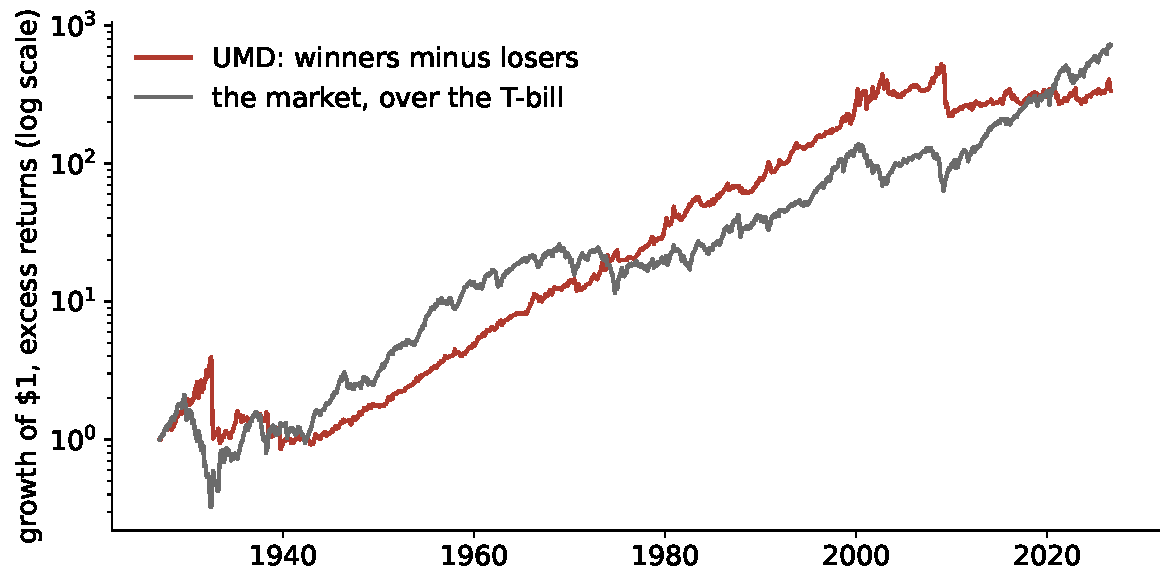
\includegraphics{figures/mom_umd_vs_market.pdf}}
\end{column}
\begin{column}{0.38\textwidth}
\begin{itemize}
\item Every month: buy last year's winners, short last year's losers
\vskip 8pt
\item \$1 in 1927 grows to \textcolor{red}{\$335}. The market: \$719
\vskip 8pt
\item Same Sharpe ratio as the market: 0.45
\end{itemize}
\end{column}
\end{columns}
\vskip 6pt
\centering Should this work?
\vskip 4pt
\pollbox{red}{\textbf{A}\ \ No: everyone can see it} \hfill
\pollbox{gray}{\textbf{B}\ \ Yes: it is risky} \hfill
\pollbox{blue}{\textbf{C}\ \ Yes: people are slow}
\end{frame}

%------------------------------------------------------------------ 3
\begin{frame}{The rule}
\vskip 6pt
\begin{center}
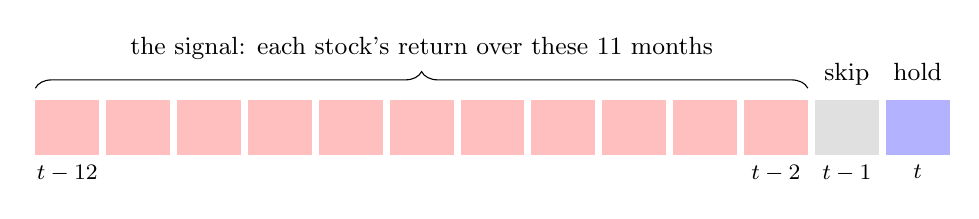
\begin{tikzpicture}[x=0.9cm, y=1cm]
\foreach \i in {0,...,10} { \fill[red!25] (\i,0) rectangle +(0.9,0.7); }
\fill[black!12] (11,0) rectangle +(0.9,0.7);
\fill[blue!30] (12,0) rectangle +(0.9,0.7);
\node[below] at (0.45,0) {\footnotesize $t-12$};
\node[below] at (10.45,0) {\footnotesize $t-2$};
\node[below] at (11.45,0) {\footnotesize $t-1$};
\node[below] at (12.45,0) {\footnotesize $t$};
\draw[decorate, decoration={brace, amplitude=6pt}] (0,0.85) -- (10.9,0.85)
  node[midway, above=7pt] {\small the signal: each stock's return over these 11 months};
\node[anchor=base] at (11.45,0.95) {\small skip};
\node[anchor=base] at (12.45,0.95) {\small hold};
\end{tikzpicture}
\end{center}
\vskip 14pt
\begin{itemize}
\item Rank every stock on the signal. Buy the top 10\%, short the bottom 10\%.
\vskip 10pt
\item Do it again next month
\vskip 10pt
\item Why skip last month? Last month's winners tend to \textcolor{red}{reverse}. Hold that thought.
\end{itemize}
\end{frame}

%------------------------------------------------------------------ 4
\begin{frame}{Winners beat losers, and the losers do most of the work}
\begin{center}
\adjustbox{max width=\textwidth, max height=0.62\textheight}{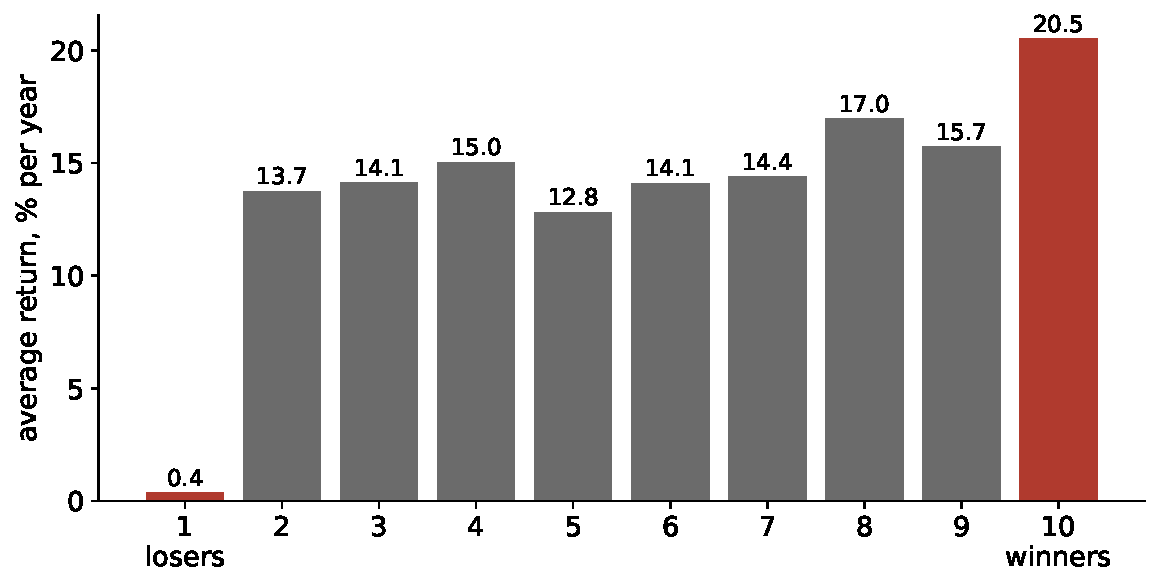
\includegraphics{figures/mom_deciles.pdf}}
\end{center}
\begin{itemize}
\item Top minus bottom decile: \textcolor{red}{20\% a year}, Sharpe ratio 1.03 (our panel, 1981--2000, value-weighted)
\item The middle deciles earn about 13.5\%. The losers earn 0.4\%.
\end{itemize}
\end{frame}

%------------------------------------------------------------------ 5
\begin{frame}{Adjusting for risk makes it bigger}
\[ UMD_t \;=\; \alpha \;+\; \beta\,\big(R^{m}_t - r^{f}_t\big) \;+\; \varepsilon_t \]
{\small $UMD_t$: winners minus losers in month $t$ \qquad $R^{m}_t - r^{f}_t$: the market over the T-bill}
\vskip 8pt
\begin{center}
\renewcommand{\arraystretch}{1.4}
\begin{tabular}{lccc}
\toprule
UMD, 1927--2026 & average return & $\alpha$ & $\beta$ \\
\midrule
per year & 7.4\% & \textcolor{red}{9.9\%} \ (t = 6.4) & $-0.30$ \\
\bottomrule
\end{tabular}
\end{center}
\vskip 6pt
\begin{itemize}
\item The losers are the stocks that fell with the market. Short them and you are short the market.
\end{itemize}
\vskip 6pt
\begin{beamercolorbox}[rounded=true,sep=8pt,center]{box1}
Momentum's alpha is larger than its average return
\end{beamercolorbox}
\end{frame}

%------------------------------------------------------------------ 6
\begin{frame}{The fourth factor}
\begin{itemize}
\item Carhart (1997) added UMD to the market, size and value
\vskip 10pt
\item Since then, a new strategy has to beat momentum too:
\end{itemize}
\[ r_t \;=\; \alpha \;+\; \beta_{m}\,\big(R^{m}_t - r^{f}_t\big) \;+\; \beta_{u}\,UMD_t \;+\; \varepsilon_t \]
\vskip 4pt
\begin{itemize}
\item $\beta_u$ near 1 and $\alpha$ near 0: the strategy is momentum under another name
\vskip 10pt
\item Today we ask it of every version: \textcolor{red}{is it anything more than UMD?}
\end{itemize}
\end{frame}

%------------------------------------------------------------------ 7
\begin{frame}{Horizon matters}
\begin{center}
\adjustbox{max width=\textwidth, max height=0.62\textheight}{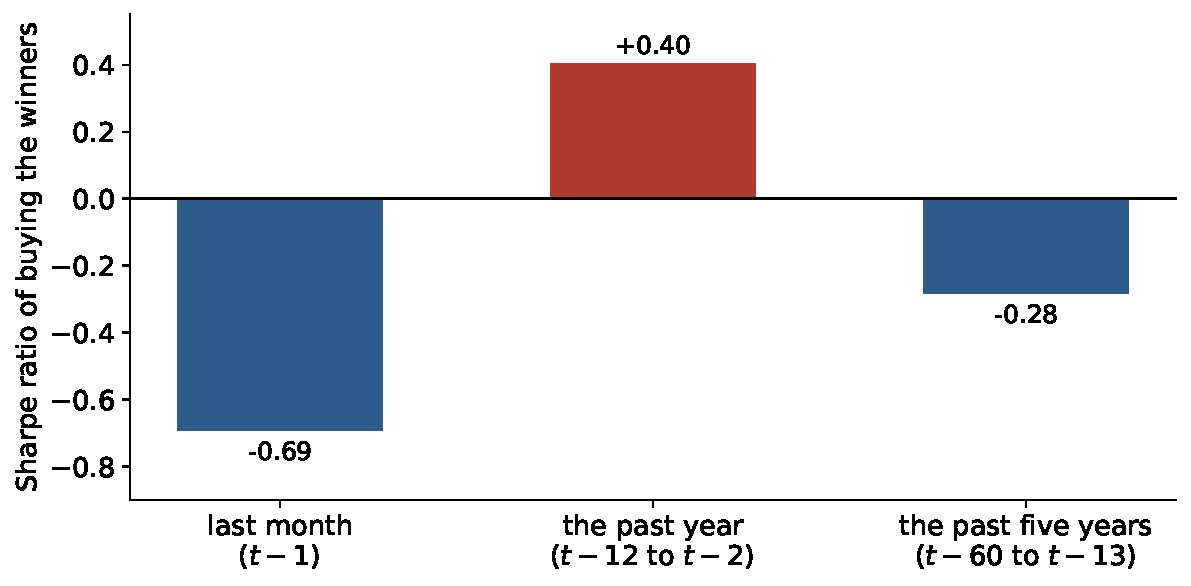
\includegraphics{figures/mom_horizons.pdf}}
\end{center}
\begin{itemize}
\item Last month reverses. The past year continues. The past five years reverse.
\item That is why the signal skips $t-1$ {\small (stocks, 1931--2026, Fama--French factors)}
\end{itemize}
\end{frame}

%================================================================== WHY
%------------------------------------------------------------------ 8
\begin{frame}{Is it risk?}
\begin{itemize}
\item A risk premium is pay for losing money in bad times
\vskip 12pt
\item Momentum does the opposite. In the worst third of market months UMD earns \textcolor{red}{+1.3\%} a month; in the best third, $-0.6\%$
\vskip 12pt
\item And the winners have just gone up: if anything they got safer, not riskier
\end{itemize}
\vskip 14pt
\centering So the simple risk story does not work
\end{frame}

%------------------------------------------------------------------ 9
\begin{frame}{Or is it behavior?}
\begin{itemize}
\item \textbf{Underreaction}: news gets into prices slowly
\vskip 10pt
\item \textbf{The disposition effect}: investors sell winners too soon and hold on to losers, so prices adjust in steps (Frazzini 2006)
\vskip 10pt
\item \textbf{Stronger where news travels slowly}: small stocks, few analysts (Hong, Lim and Stein 2000)
\end{itemize}
\vskip 14pt
\begin{beamercolorbox}[rounded=true,sep=8pt,center]{box1}
Then why has no one traded it away? Because it crashes. Hold that thought too.
\end{beamercolorbox}
\end{frame}

%------------------------------------------------------------------ 10
\begin{frame}{It survives out of sample}
\begin{center}
\renewcommand{\arraystretch}{1.4}
\begin{tabular}{llccc}
\toprule
UMD & & average & Sharpe & CAPM $\alpha$ \\
\midrule
1927--1964 & before the paper's data & 7.7\% & 0.41 & 11.9\% \ (t = 4.6) \\
1965--1989 & the paper's sample & 9.9\% & 0.80 & \phantom{1}9.8\% \ (t = 4.0) \\
1990--2026 & after publication & 5.3\% & 0.33 & \textcolor{red}{\phantom{1}7.9\%} \ (t = 3.0) \\
\bottomrule
\end{tabular}
\end{center}
\vskip 10pt
\begin{itemize}
\item Weaker since publication, still there
\vskip 8pt
\item And in other markets: equity indices, currencies, bonds, commodities. All asset classes combined: a Sharpe ratio of 0.81, 1972--2010 (Asness, Moskowitz and Pedersen 2013)
\end{itemize}
\end{frame}

%================================================================== THE MANY MOMENTA
%------------------------------------------------------------------ 11
\begin{frame}[label=many]{So everyone built a version}
\footnotesize
\renewcommand{\arraystretch}{1.3}
\begin{center}
\begin{tabular}{lll}
\toprule
variation & what changes & paper \\
\midrule
cross-sectional & the original: rank on $t-12$ to $t-2$ & Jegadeesh and Titman 1993 \\
earnings momentum & rank on the announcement return & Chan, Jegadeesh, Lakonishok 1996 \\
industry momentum & rank industries, not stocks & Moskowitz and Grinblatt 1999 \\
slow diffusion & stronger where coverage is thin & Hong, Lim and Stein 2000 \\
52-week high & distance from the 52-week high & George and Hwang 2004 \\
residual momentum & momentum in model residuals & Blitz, Huij and Martens 2011 \\
the echo & months 7--12 only & Novy-Marx 2012 \\
time-series momentum & your own past return, not a rank & Moskowitz, Ooi, Pedersen 2012 \\
everywhere & bonds, currencies, commodities & Asness, Moskowitz, Pedersen 2013 \\
risk-managed & scale by trailing volatility & Barroso and Santa-Clara 2015 \\
\bottomrule
\end{tabular}
\end{center}
\hfill \hyperlink{appendix_many}{\beamerbutton{The full list}}
\end{frame}

%------------------------------------------------------------------ 12
\begin{frame}{Many papers. How many trades?}
\begin{center}
\renewcommand{\arraystretch}{1.4}
\begin{tabular}{lccc}
\toprule
1980--2000 & Sharpe & corr.\ with 12-month momentum & $\alpha$ on market + UMD \\
\midrule
6-month momentum & 0.61 & 0.79 & $-0.2\%$ \ (t = $-0.1$) \\
residual momentum & 0.64 & 0.53 & \phantom{$-$}2.5\% \ (t = 1.0) \\
earnings momentum & 1.17 & 0.24 & \textcolor{red}{10.1\%} \ (t = 4.5) \\
\bottomrule
\end{tabular}
\end{center}
\vskip 10pt
\begin{itemize}
\item Six-month momentum is UMD again. Earnings momentum is a different trade.
\vskip 8pt
\item You cannot tell from the name. Run the regression.
\end{itemize}
\end{frame}

%------------------------------------------------------------------ 13
\begin{frame}{Industries}
Moskowitz and Grinblatt (1999): \emph{Do industries explain momentum?}
\vskip 10pt
\begin{itemize}
\item Industries have momentum too: buy last year's best industries, short the worst
\vskip 10pt
\item Their claim: much of stock momentum is industry momentum
\vskip 10pt
\item If so, momentum is a bet on a few sectors, and less diversified than it looks
\end{itemize}
\vskip 14pt
\centering Our question: industry momentum since 1927. Is it anything more than UMD?
\end{frame}

%================================================================== THE NOTEBOOK
\begin{frame}{Now: the notebook}
\vskip 2pt
\begin{beamercolorbox}[rounded=true,sep=7pt,center]{box1}
\textbf{Notebook: Momentum} \ --- \ one strategy, three ways, the same two regressions
\end{beamercolorbox}
\vskip 10pt
\begin{enumerate}
\item \textbf{Stock momentum.} Four steps on our panel, then the CAPM and the market + UMD regressions.
\vskip 5pt
\item \textbf{Industry momentum, 1927--2026.} Build it with AI, check it, then the same two regressions.
\end{enumerate}
\vskip 8pt
{\small \textbf{Bring back:} is industry momentum a different trade from stock momentum? \\[2pt]
Stop at \textbf{Back to the slides}; the challenge after it is homework.}
\end{frame}
%================================================================== BACK TO THE SLIDES

%------------------------------------------------------------------ 15
\begin{frame}{Industry momentum is mostly UMD}
\begin{center}
\renewcommand{\arraystretch}{1.4}
\begin{tabular}{lccc}
\toprule
 & CAPM $\alpha$ & $\alpha$ on market + UMD & UMD $\beta$ \\
\midrule
stock momentum, 1981--2000 & 19.0\% \ (t = 4.3) & \phantom{1}5.1\% \ (t = 2.7) & 1.45 \\
industry momentum, 1927--2026 & 13.2\% \ (t = 5.9) & \textcolor{red}{\phantom{1}2.9\%} \ (t = 1.8) & 1.05 \\
\bottomrule
\end{tabular}
\end{center}
\vskip 10pt
\begin{itemize}
\item Over a century, the industry bet and the stock bet are mostly one trade (correlation 0.74)
\vskip 8pt
\item Our stock deciles load more than 1 on UMD because they are more extreme than UMD's 30/70 split
\end{itemize}
\end{frame}

%================================================================== CRASHES
%------------------------------------------------------------------ 16
\begin{frame}{Both crash, at the same time}
\begin{center}
\adjustbox{max width=\textwidth, max height=0.6\textheight}{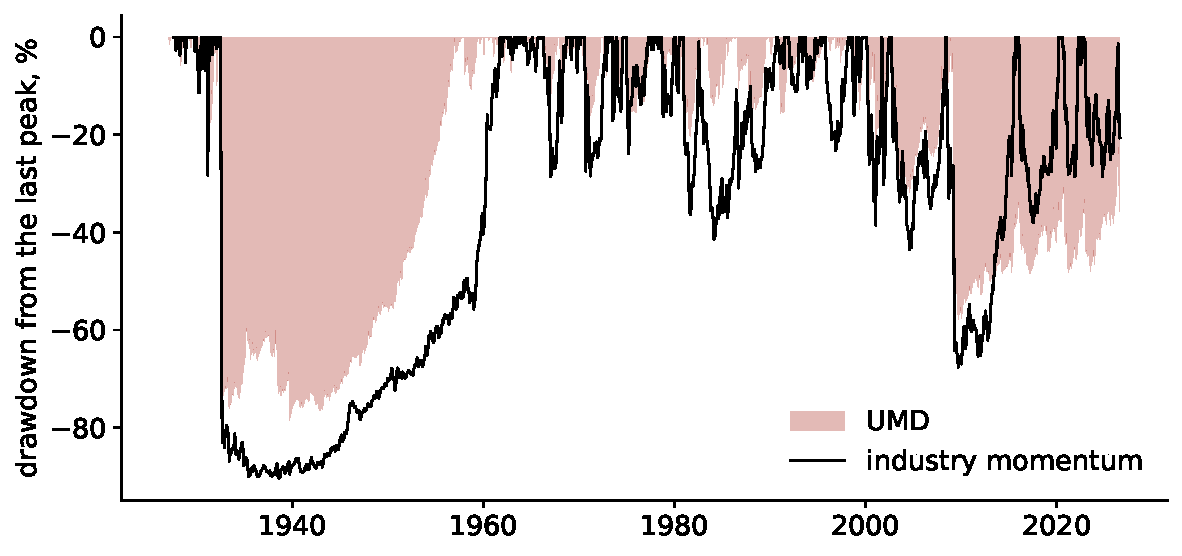
\includegraphics{figures/mom_crashes.pdf}}
\end{center}
\begin{itemize}
\item 1932: UMD \textcolor{red}{$-65\%$}, industry momentum $-71\%$. The market: $-9\%$.
\item 2009: UMD \textcolor{red}{$-53\%$}, industry momentum $-50\%$. The market: $+29\%$.
\end{itemize}
\end{frame}

%------------------------------------------------------------------ 17
\begin{frame}{Why it crashes}
\begin{center}
\renewcommand{\arraystretch}{1.4}
\begin{tabular}{lccc}
\toprule
UMD, 1927--2026 & months & market $\beta$ & average return \\
\midrule
after a two-year bear market & 191 & \textcolor{red}{$-0.68$} & $-9.3\%$ a year \\
after a two-year bull market & 1,005 & \phantom{$-$}0.01 & $+10.5\%$ a year \\
\bottomrule
\end{tabular}
\end{center}
\vskip 10pt
\begin{itemize}
\item After a crash, the losers are the stocks that fell the most: high-beta stocks
\vskip 8pt
\item Short them, and you are short the rebound. In the months the market rose after a bear market, UMD lost 4.1\% a month
\vskip 8pt
\item Momentum is short a call on the market's recovery (Daniel and Moskowitz 2016)
\end{itemize}
\end{frame}

%================================================================== VOLATILITY MANAGEMENT
%------------------------------------------------------------------ 18
\begin{frame}{After a volatile month: more risk, no more return}
\begin{center}
\adjustbox{max width=\textwidth, max height=0.6\textheight}{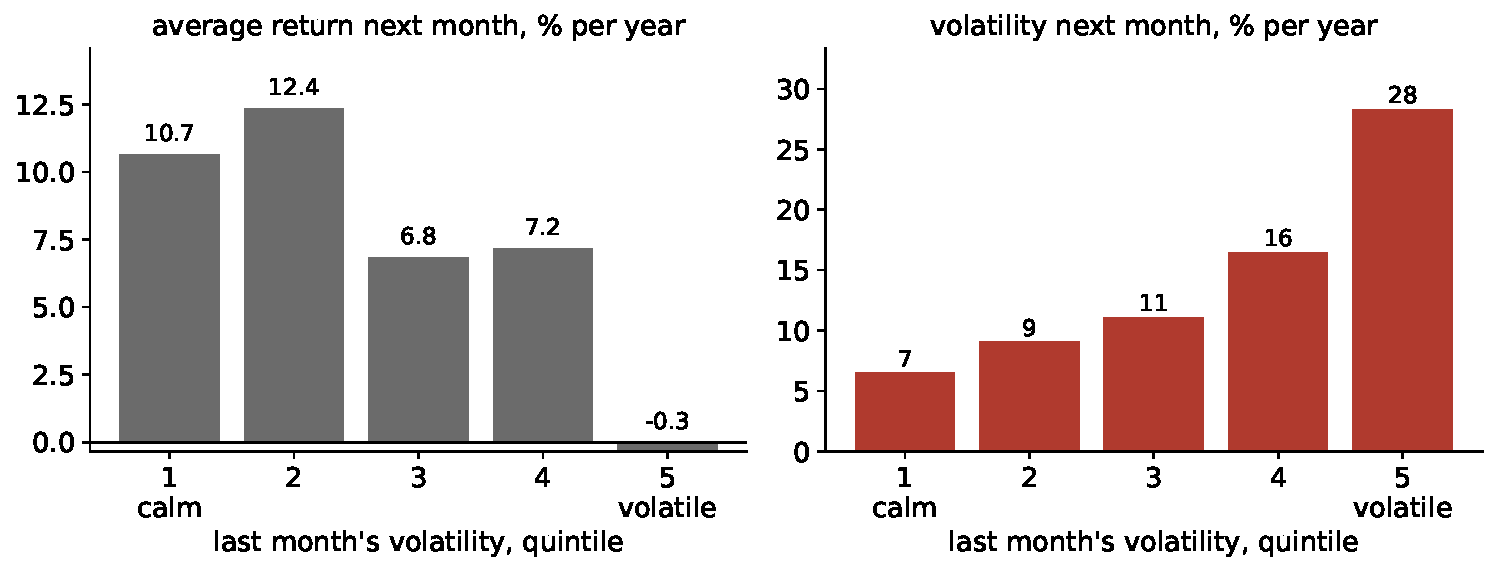
\includegraphics{figures/mom_vol_quintiles.pdf}}
\end{center}
\begin{itemize}
\item Volatility persists: this month's variance tracks last month's (correlation 0.78, in logs)
\item The average return does not follow. Sharpe ratio: 1.6 after the calmest months, \textcolor{red}{0} after the most volatile
\end{itemize}
\end{frame}

%------------------------------------------------------------------ 19
\begin{frame}[label=managed]{So hold less after a volatile month}
\[ UMD^{\sigma}_t \;=\; \frac{c}{RV_{t-1}}\; UMD_t \]
\vskip 2pt
\begin{itemize}
\item $RV_{t-1}$: the variance of momentum's daily returns last month
\vskip 6pt
\item $c$: a constant, set so $UMD^{\sigma}$ has the same volatility as UMD. It sets the scale, not the Sharpe ratio
\vskip 6pt
\item Barroso and Santa-Clara (2015); Moreira and Muir (2017)
\end{itemize}
\vskip 12pt
\begin{beamercolorbox}[rounded=true,sep=8pt,center]{box1}
You do not need to forecast returns. Only volatility, and volatility is predictable.
\end{beamercolorbox}
\vskip 4pt
\hfill \hyperlink{appendix_managed}{\beamerbutton{Details}}
\end{frame}

%------------------------------------------------------------------ 20
\begin{frame}{Twice the Sharpe ratio, half the drawdown}
\begin{columns}[c]
\begin{column}{0.60\textwidth}
\adjustbox{max width=\textwidth}{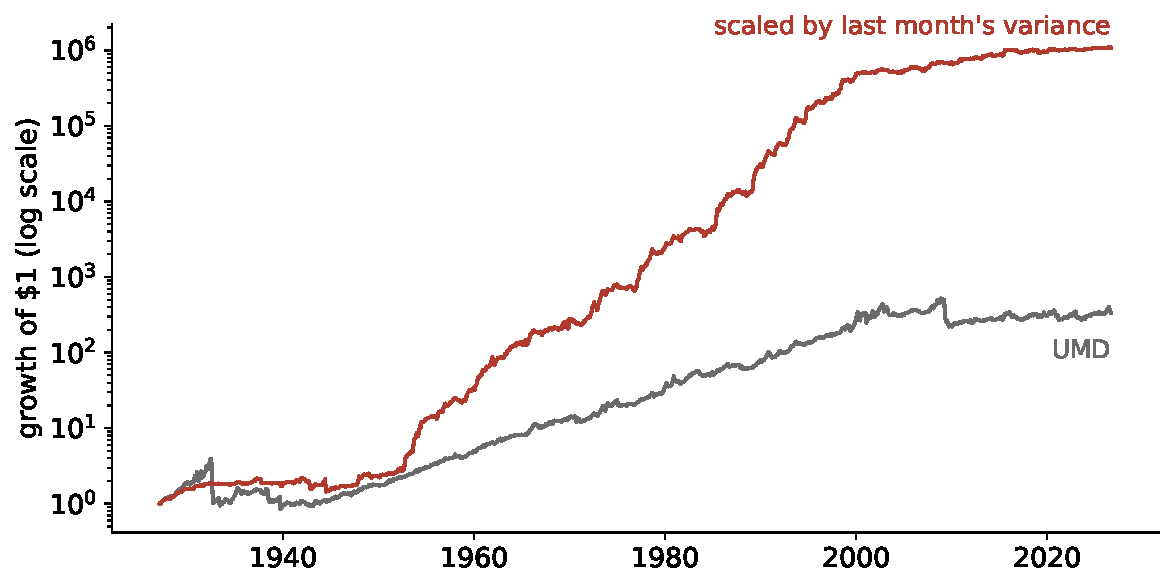
\includegraphics{figures/mom_vol_managed.pdf}}
\end{column}
\begin{column}{0.38\textwidth}
\begin{itemize}
\item Sharpe ratio: 0.45 $\to$ \textcolor{red}{0.94}
\vskip 8pt
\item Worst drawdown: $-78\%$ $\to$ $-33\%$
\vskip 8pt
\item 1932: $-0.5\%$. \ 2009: $-0.2\%$.
\vskip 8pt
\item $\alpha$ on market + UMD: 10.4\% a year (t = 7.1)
\end{itemize}
\end{column}
\end{columns}
\vskip 8pt
{\small Same volatility as UMD, 1927--2026}
\end{frame}

%------------------------------------------------------------------ 21
\begin{frame}{The catch}
\begin{itemize}
\item \textbf{Leverage.} The position is above 2$\times$ in a quarter of months, and above 8$\times$ in the calmest 1\%
\vskip 10pt
\item \textbf{Trading.} The position moves by 0.9 a month on average
\vskip 10pt
\item \textbf{Hindsight.} $c$ uses the whole sample. It does not change the Sharpe ratio, but it does set the leverage
\end{itemize}
\vskip 14pt
\centering Cap the position at 2$\times$: Sharpe ratio \textcolor{red}{0.97}, worst drawdown $-20\%$
\end{frame}

%------------------------------------------------------------------ 22
\begin{frame}{What to take away}
\begin{itemize}
\item Buy the past year's winners, skip last month: a century of returns, with a negative beta
\vskip 10pt
\item Not a risk premium in the usual sense. Most likely, slow reaction to news
\vskip 10pt
\item Many versions, fewer trades: regress on UMD before you believe a new one
\vskip 10pt
\item It crashes in rebounds, when volatility is high. Scale by last month's variance.
\end{itemize}
\vskip 14pt
{\small \textbf{Homework:} the challenge at the end of the notebook. Volatility-managed industry momentum.}
\end{frame}

%================================================================== appendix
\appendix
\begin{frame}
\begin{center}
{\Large Appendix}
\end{center}
\end{frame}

\begin{frame}[label=appendix_many]{A1: The many momenta, the longer list}
\scriptsize
\renewcommand{\arraystretch}{1.05}
\begin{center}
\begin{tabular}{P{2.8cm}P{4.8cm}P{4.9cm}}
\toprule
variation & what changes & paper \\
\midrule
cross-sectional (12,1) & the original & Jegadeesh and Titman 1993, \emph{JF} \\
UMD as a factor & a benchmark, not a trade & Carhart 1997, \emph{JF} \\
earnings momentum & the signal is the announcement return, not the price & Chan, Jegadeesh and Lakonishok 1996, \emph{JF} \\
industry momentum & rank industries, not stocks & Moskowitz and Grinblatt 1999, \emph{JF} \\
slow information diffusion & stronger where coverage is thin & Hong, Lim and Stein 2000, \emph{JF} \\
volume-conditioned & interact the signal with turnover & Lee and Swaminathan 2000, \emph{JF} \\
beta-hedged & strip out the time-varying market exposure & Grundy and Martin 2001, \emph{RFS} \\
52-week high & distance from a high, not a cumulative return & George and Hwang 2004, \emph{JF} \\
residual momentum & momentum in Fama--French residuals & Blitz, Huij and Martens 2011, \emph{JEmpFin} \\
the echo & months 7--12 only, not 2--12 & Novy-Marx 2012, \emph{JFE} \\
time-series momentum & your own past return, not a relative rank & Moskowitz, Ooi and Pedersen 2012, \emph{JFE} \\
everywhere & the same signal in bonds, FX, commodities & Asness, Moskowitz and Pedersen 2013, \emph{JF} \\
frog in the pan & gradual news beats sudden news & Da, Gurun and Warachka 2014, \emph{RFS} \\
risk-managed & scale the position by trailing volatility & Barroso and Santa-Clara 2015, \emph{JFE} \\
crashes & when and why it fails & Daniel and Moskowitz 2016, \emph{JFE} \\
\bottomrule
\end{tabular}
\end{center}
\hfill \hyperlink{many}{\beamerreturnbutton{Back}}
\end{frame}

\begin{frame}[label=appendix_managed]{A2: How the volatility-managed version is built}
\begin{itemize}
\item Daily UMD returns from Ken French's library; for each month, $RV_t = \sum_{d \in t} (r_d - \bar r_t)^2$
\vskip 8pt
\item Weight for month $t$: $c / RV_{t-1}$, known at the start of the month
\vskip 8pt
\item $c$ makes the managed series as volatile as UMD over 1927--2026
\vskip 8pt
\item Weight on UMD: median 0.84, 90th percentile 3.7, 99th percentile 8.1
\vskip 8pt
\item CAPM $\alpha$: 15.4\% a year (t = 9.4). On market + UMD: 10.4\% (t = 7.1), UMD $\beta$ 0.51
\end{itemize}
\vskip 4pt
\hfill \hyperlink{managed}{\beamerreturnbutton{Back}}
\end{frame}

\begin{frame}{A3: Data}
\small
\begin{itemize}
\item \textbf{Factors}: market, T-bill, UMD, short- and long-term reversal; monthly and daily, July 1926 to August 2026. Ken French's data library.
\vskip 8pt
\item \textbf{Industries}: the 49 value-weighted industry portfolios, monthly and daily, from the same library. Industry momentum: rank on $t-12$ to $t-2$, the top 5 minus the bottom 5, equal-weighted.
\vskip 8pt
\item \textbf{Stocks}: our CRSP panel, 1980--2000. Common stocks on NYSE, AMEX and Nasdaq; deciles on NYSE breakpoints, value-weighted.
\vskip 8pt
\item \textbf{The momentum variants}: the published long-shorts from the factor-zoo lecture, 1980--2000.
\end{itemize}
\end{frame}

\end{document}
